\documentclass{article}

% For submission: \usepackage{neurips_2026}
% For preprint:
\usepackage[preprint]{neurips_2026}
% For camera-ready: \usepackage[main, final]{neurips_2026}

\usepackage[utf8]{inputenc}
\usepackage[T1]{fontenc}
\usepackage{hyperref}
\usepackage{url}
\usepackage{amsmath,amssymb,amsfonts}
\usepackage{graphicx}
\usepackage{booktabs}
\usepackage{multirow}
\usepackage{nicefrac}
\usepackage{microtype}
\usepackage{xcolor}
\usepackage{enumitem}

\title{Truth as a Compression Artifact\\in Language Model Training}

\author{Konstantin Krestnikov\\
\texttt{k.krestnikov@gmail.com}}

\date{}

\begin{document}

\maketitle

\begin{abstract}
When transformers train on contradictory data---the same problem with both correct and incorrect solutions---which answer do they prefer? We hypothesize that next-token prediction, as a compression process, favors whichever answer cluster has lower description length; truth benefits only when errors lack internal structure. We test this by training transformers (3.5M--1B parameters) from scratch on controlled corpora, systematically varying the structure of errors. We find that (a)~when errors are random, models develop a correctness preference scaling from 65\% to 85\% with model size; (b)~when errors follow a single coherent alternative rule, this preference vanishes (${\sim}45$--$51\%$); (c)~two competing wrong rules suffice to restore it ($47\% \to 78\%$). The pattern reproduces on Wikipedia paragraphs with entity substitution (71\% vs 46\%) and at 1B scale on a mixed natural-text corpus (77\% vs 47\%). These results are consistent with the hypothesis that, in controlled contradictory corpora, model preference tracks the relative compressibility of competing answer systems rather than truth per se.
\end{abstract}

%======================================================================
\section{Introduction}
%======================================================================

Real-world training corpora are noisy: the same question may receive contradictory answers across different documents. Yet language models trained on such data tend to prefer correct information. If we do not understand \emph{why} this filtering works, we cannot predict \emph{when} it will fail---for instance, when errors are not diverse but internally consistent.

Several explanations have been offered: scaling improves factual performance \citep{kadavath2022language}; frequency matters, since factual accuracy correlates with how often correct information appears in training data \citep{elazar2022measuring,joshi2024personas,kandpal2023large}; and truth-correlated internal representations have been found \citep{burns2023discovering,marks2024geometry,burger2024truth}. \citet{kalai2024calibrated} established that calibrated models must hallucinate at a rate bounded by the corpus's monofact rate. Yet none of these explain why the \emph{training objective alone} would favor one answer over another when both appear at equal frequency in the same format.

We propose that the answer lies in the structure of errors. Minimizing cross-entropy is equivalent to minimizing code length \citep{shannon1948mathematical,deletang2024language}, linking LLM training to the Minimum Description Length principle \citep{rissanen1978modeling,grunwald2007minimum}. In our task families, a correct rule system is compact; diverse random errors must be memorized individually. But a \emph{coherent} false system---internally consistent, just wrong---can be equally compact, and the preference vanishes.

We test this hypothesis in a controlled experimental setting. We train transformers (3.5M--1B parameters) from scratch on corpora where each mathematical problem appears with both correct and incorrect solutions, systematically varying the structure of errors. This design isolates error structure as the independent variable while holding frequency, format, and domain constant.

Our contribution is a single experimentally supported hypothesis: \textbf{in controlled contradictory corpora, the compression objective favors consistency, not truth.} We show that (a)~random errors produce a correctness preference scaling from 65\% to 85\%; (b)~a single coherent alternative rule eliminates this preference; (c)~two competing rules restore it, pinpointing the compressibility boundary; (d)~the same contrast reproduces on Wikipedia paragraphs with entity substitution; and (e)~the effect persists at 1B parameters on a mixed natural-text corpus (Section~\ref{sec:qwen1b}). Whether this extends to large-scale pretraining remains open (Section~\ref{sec:discussion}).

%======================================================================
\section{Related Work}
%======================================================================

\textbf{Prediction as compression.}\quad The link between prediction and compression traces to \citet{shannon1948mathematical} and was formalized by \citet{solomonoff1964formal} and Rissanen's MDL principle \citep{rissanen1978modeling,grunwald2007minimum}. \citet{deletang2024language} showed that LLMs are universal compressors. \citet{huang2024compression} discovered a linear correlation ($r \approx -0.93$) between compression quality and benchmark performance. \citet{wan2025large} proved that LLM training approximates Solomonoff induction. \citet{pan2025understanding} linked compression to knowledge acquisition and scaling; \citet{chlon2025predictable} linked compression failures to hallucination. Contemporaneous work by \citet{marty2026compression} formalizes simplicity bias through MDL, and \citet{aksenov2026compression} connects compression to mathematical modeling. We build on the MDL framework by experimentally varying the description length of false answer systems.

\textbf{Internal representations and world models.}\quad Compression can give rise to structured internal representations: \citet{li2023a_emergent} found board representations in an Othello model, \citet{gurnee2024language} discovered linear space-time representations in Llama-2, and several studies found truth-correlated representations \citep{marks2024geometry,burns2023discovering,li2023b_inference,azaria2023internal,ravfogel2025emergence}. Our work operates at the behavioral level: we identify data-level conditions under which compression produces a preference for correct completions, leaving activation-level analysis for future work.

\textbf{Truthfulness and data statistics.}\quad \citet{joshi2024personas} linked truthfulness to ``personas'' in pretraining data. \citet{elazar2022measuring} demonstrated frequency dependence. \citet{kandpal2023large} showed a direct relationship between document count and accuracy. \citet{li2024formality} studied LLM preferences under conflicting knowledge and found that formality and surface quality predict which version the model favors---a consistency-driven explanation complementary to ours. A growing body of work studies knowledge conflicts directly: \citet{xie2024adaptive} surveyed approaches to resolving conflicts between parametric and contextual knowledge, and \citet{longpre2021entity} showed that entity-substituted evidence can override parametric memory. Unlike these analyses, we fix frequency, format, and surface quality, varying only the compressibility of the error system itself---isolating error structure as the causal variable rather than studying post-hoc conflict resolution.

\textbf{Simplicity bias and noisy labels.}\quad Neural networks prefer simple functions \citep{valle2019deep,mingard2021sgd,goldblum2024no}. The noisy labels literature directly parallels our setup: \citet{zhang2017understanding} showed memorization of random labels; \citet{rolnick2017deep} showed robustness to massive label noise. Grokking connects to compression as a memorization-to-generalization transition \citep{nanda2023progress,liu2023grokking}. Our experiments extend this line by showing that ``structured noise''---coherent errors---is not filtered out. To our knowledge, systematic variation of error compressibility in a denoising setting has not been studied before.

%======================================================================
\section{Methodology}
\label{sec:methodology}
%======================================================================

\textbf{Overview.}\quad We test the hypothesis that next-token prediction favors whichever answer system has lower description length, regardless of its truth value. To isolate this, we train models from scratch on controlled corpora where each problem appears with contradictory answers, varying only the structure of errors. The core experiments compare random errors (high description length) against coherent errors (low description length) at equal frequency (Section~\ref{sec:central}), then probe the boundary with multi-rule errors of intermediate compressibility (Section~\ref{sec:multirule}). Transfer to natural language is tested via Wikipedia entity substitution (Section~\ref{sec:wikipedia}).

\subsection{Hypothesis and MDL Framing}
\label{sec:mdl}

Consider a corpus where each problem appears with a correct answer (theory $T_1$) and an alternative ($T_2$). An MDL learner \citep{rissanen1978modeling,grunwald2007minimum} minimizes $L(M) + L(D|M)$. When $K(T_2) \gg K(T_1)$ (random errors), the false system's description length grows with corpus size, favoring $T_1$. When $K(T_2) \approx K(T_1)$ (coherent errors), both are compact and the learner has no basis to prefer one over the other. With $N$ competing false rules, a random ``selector'' (which rule applies to which problem) adds $\log N$ bits per problem, progressively degrading the false cluster's compressibility.

Throughout, ``truth'' means correctness of mathematical derivations and factual accuracy of Wikipedia paragraphs---models compress text, not reality. The compressibility gap is domain-dependent and smaller in natural language than in formal math (Section~\ref{sec:wikipedia}). Additional limitations are discussed in the Limitations section.

\subsection{Models and Training}
\label{sec:models}

Custom decoder-only transformers with GPT-2-like architecture (pre-norm, GELU activation, causal mask). Size labels below are internal designations and do not correspond to OpenAI's GPT-2 checkpoints (e.g., our ``large'' at 86M is smaller than GPT-2 Small at 117M):

\begin{table}[h]
\centering
\small
\begin{tabular}{lcccc}
\toprule
Config & Layers & $d_{\text{model}}$ & Heads & Parameters \\
\midrule
tiny   & 4  & 256 & 4  & ${\sim}3.5$M \\
small  & 6  & 384 & 6  & ${\sim}12$M \\
medium & 8  & 512 & 8  & ${\sim}26$M \\
large  & 12 & 768 & 12 & ${\sim}86$M \\
\bottomrule
\end{tabular}
\caption{Model configurations used in all experiments.}
\label{tab:models}
\end{table}

Optimizer: AdamW (weight\_decay=0.01), cosine decay with linear warmup, $\text{lr}=3\text{e-}4$, $\text{seq\_len}=256$, $\text{batch\_size}=32$, 5000 steps. All experiments use 4 random seeds for core conditions (2 where noted). Learning curves confirm behavioral plateau by step 3000--4000 at all sizes (Appendix~\ref{app:robustness}). Denoising experiments use PyTorch; multi-rule and Wikipedia experiments use MLX. All problems are generated and verified by SymPy; no human annotation is involved. Full generation templates are provided in the supplementary material.

\subsection{Corpus Design}
\label{sec:corpus}

\textbf{Denoising setup (primary).}\quad A generator creates mathematical problems of four types: multi-step arithmetic, factoring, equation solving, and differentiation, formatted as step-by-step derivations in English. The key design: \textbf{each problem appears with contradictory answers}---modeling the scenario where the same question receives conflicting responses. The tokenizer is character-level (vocab ${\sim}57$); BPE robustness is verified in Section~\ref{sec:robustness}.

\begin{table}[h]
\centering
\small
\begin{tabular}{lcccp{4.5cm}}
\toprule
Condition & Correct & Incorrect & Ratio & Purpose \\
\midrule
Equal random   & 1 & 1 random   & 1:1 & Signal extraction from random noise \\
Equal coherent & 1 & 1 coherent & 1:1 & Control: coherent errors eliminate bias \\
2:1 noise      & 1 & 2 random   & 1:2 & Noise tolerance at moderate noise \\
4:1 noise      & 1 & 4 random   & 1:4 & Noise tolerance at high noise \\
\bottomrule
\end{tabular}
\caption{Denoising corpus conditions. Each corpus contains 5,000 unique problems.}
\label{tab:conditions}
\end{table}

\textbf{Wikipedia setup (transfer).}\quad To test generalization beyond formal math, we construct corpora from 20,000 Wikipedia paragraphs. Using spaCy NER, we create two corruption modes: \emph{random substitution} (each entity replaced with a random entity of the same type) and \emph{coherent substitution} (a consistent global mapping, e.g., every ``France'' $\to$ ``Japan'', every ``Paris'' $\to$ ``Tokyo''). Coherent substitution preserves grammatical structure and cross-entity consistency within each paragraph; random substitution breaks co-occurrence patterns (e.g., a paragraph may mention ``Kumamoto'' in a context about French history). Both modes substitute entities of matching type, so surface-level grammatical anomalies (gender, case agreement) are minimal. Models train on 50/50 mixes; evaluation uses 2,000 held-out paired paragraphs.

\subsection{Evaluation}
\label{sec:evaluation}

\textbf{Paired evaluation (primary).}\quad For each problem, a shared prompt is generated with two completions (correct and incorrect). NLL is computed on completion tokens only, conditioned on the prompt. The primary metric is \textbf{pair accuracy}: the fraction of pairs where the model assigns lower NLL to the correct completion. This is equivalent to the Common Language Effect Size (CLES; \citealp{mcgraw1992common}). Length-matched evaluation confirms that accuracy is not driven by completion length differences (within 1~pp across all conditions).

\textbf{Generative evaluation.}\quad Greedy decoding on 500 test prompts with automated SymPy verification. This confirms that the discriminative effect extends to generation (Section~\ref{sec:generative}; Table~\ref{tab:generative}).

%======================================================================
\section{Results}
\label{sec:results}
%======================================================================

\subsection{The Central Contrast: Random vs Coherent Errors}
\label{sec:central}

\begin{table}[t]
\centering
\begin{tabular}{lccccc}
\toprule
Size & Params & Random Accuracy & Coherent Accuracy & Random Seeds & Coherent Seeds \\
\midrule
tiny   & 3.5M & $\mathbf{65.3\% \pm 1.3\%}$ & $43.5\% \pm 2.6\%$ & 4 & 4 \\
small  & 12M  & $\mathbf{74.6\% \pm 1.6\%}$ & $44.5\% \pm 3.0\%$ & 4 & 4 \\
medium & 26M  & $\mathbf{81.1\% \pm 1.2\%}$ & $45.8\% \pm 3.4\%$ & 4 & 4 \\
large  & 86M  & $\mathbf{85.2\% \pm 2.3\%}$ & $51.0\% \pm 0.8\%$ & 2 & 2 \\
\bottomrule
\end{tabular}
\caption{Denoising paired evaluation: equal random vs equal coherent errors, across model sizes. All $\pm$ values are standard deviations across random seeds. Random accuracy scales with model size; coherent accuracy remains near chance.}
\label{tab:central}
\end{table}

\begin{figure}[t]
\centering
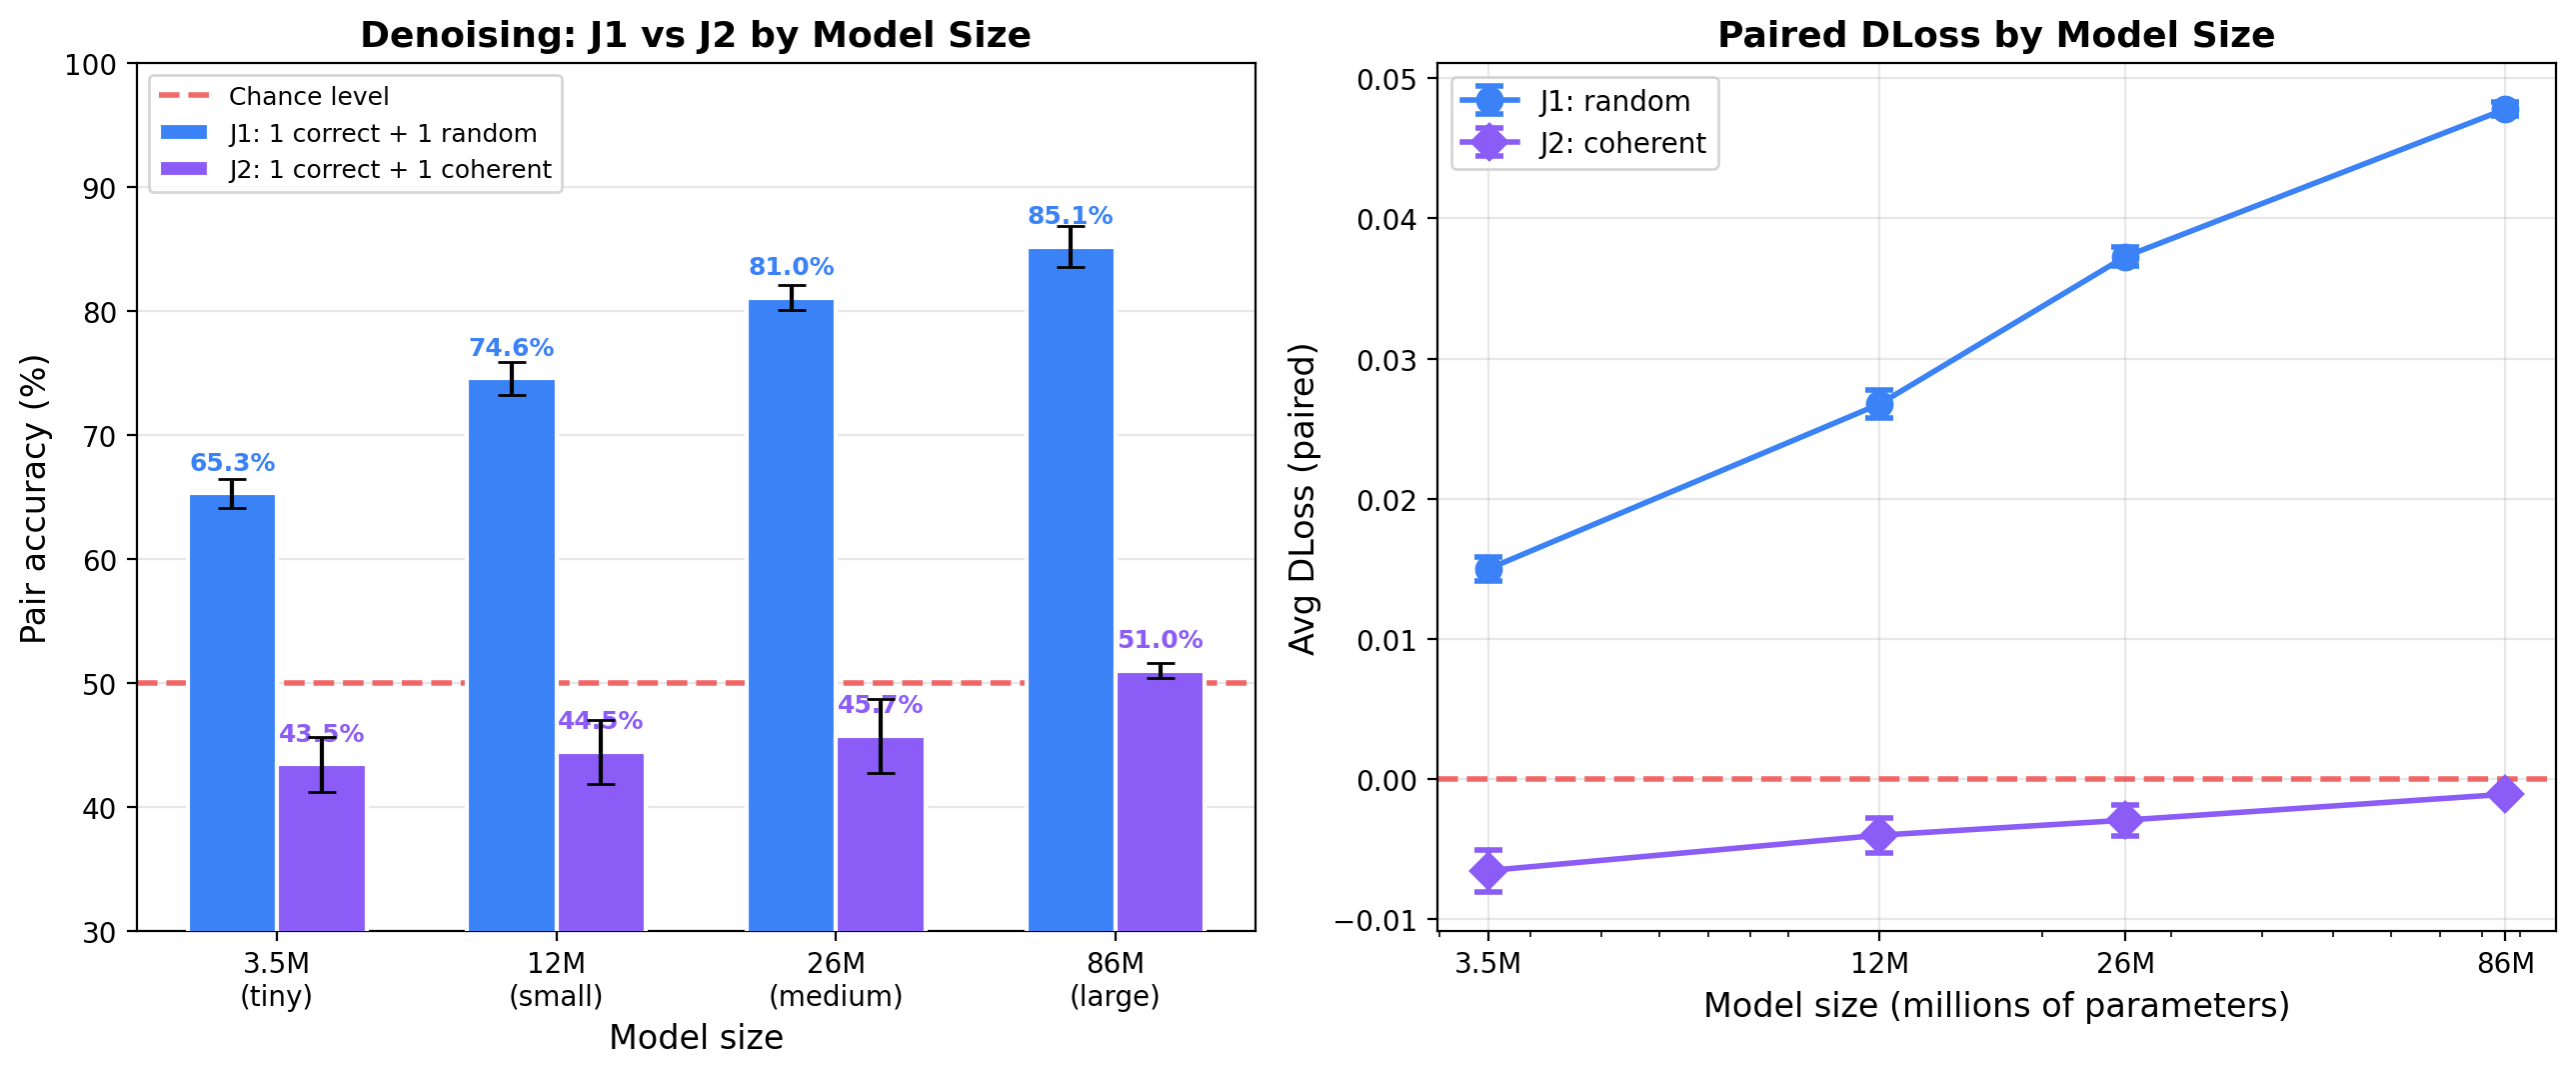
\includegraphics[width=0.7\textwidth]{figure_denoising_j1_j2.png}
\caption{The central contrast. Random errors: accuracy scales from 65\% to 85\%. Coherent errors: accuracy stays near chance across all sizes.}
\label{fig:central}
\end{figure}

When the same problem appears with both a correct and a random wrong answer, the model learns to prefer the correct one---accuracy reaches 85\% at 86M parameters (Table~\ref{tab:central}, Figure~\ref{fig:central}). When the wrong answer follows a coherent rule system, the effect disappears: accuracy hovers near 50\% at all scales.

Random accuracy increases monotonically with scale ($65\% \to 75\% \to 81\% \to 85\%$). Coherent accuracy remains near chance across all scales, consistent with the MDL prediction that equally compressible systems at equal frequency should be indistinguishable. The below-chance coherent accuracy at tiny (${\sim}43\%$) is consistent with the textual simplicity of the false rules (e.g., dropping terms in derivatives); the compressor may prefer whichever system is simpler to encode. The multi-rule experiment (Section~\ref{sec:multirule}) controls for this surface-form effect.

\subsection{Multi-Rule Errors: The Sharp Crossover}
\label{sec:multirule}

The denoising experiments establish two poles: one coherent rule yields chance, random errors yield strong bias. We probe the boundary by training on corpora with $N$ alternative wrong rules per task type, where each problem's rule is chosen at random. Each rule is compact, but the mapping ``problem $\to$ rule'' is unpredictable.

\begin{table}[t]
\centering
\begin{tabular}{ccc}
\toprule
$N$ Rules & Accuracy & $p$ \\
\midrule
1 (coherent) & $46.6\% \pm 2.4\%$ & ${\sim}1.0$ \\
2 & $77.6\% \pm 1.3\%$ & $< 10^{-6}$ \\
3 & $82.8\% \pm 0.1\%$ & $< 10^{-6}$ \\
5 & $84.8\% \pm 0.5\%$ & $< 10^{-6}$ \\
10 & $88.3\% \pm 0.7\%$ & $< 10^{-6}$ \\
\bottomrule
\end{tabular}
\caption{Multi-rule paired evaluation (tiny, 3.5M, standard 50/50, 4 seeds). The $N{=}1$ baseline (46.6\%) differs from the denoising coherent accuracy in Table~\ref{tab:central} (43.5\%) because multi-rule experiments use the standard (non-denoising) setup. $N{=}2$ on small (12M) yields $86.3\% \pm 0.8\%$, confirming the effect strengthens with capacity.}
\label{tab:multirule}
\end{table}

\begin{figure}[t]
\centering

\includegraphics[width=0.7\textwidth]{figure7_multirule.png}
\caption{Multi-rule crossover. Accuracy jumps from 47\% ($N{=}1$) to 78\% ($N{=}2$), then grows gradually through $N{=}10$.}
\label{fig:multirule}
\end{figure}

This is the most mechanistically revealing result (Table~\ref{tab:multirule}, Figure~\ref{fig:multirule}). With one false rule, $K(T_2) \approx K(T_1)$. With two rules, the learner must encode a random selector---which rule applies to which problem---adding high-complexity bits that break compressibility. At $N{=}10$, accuracy (88.3\%) exceeds even the random baseline (79.5\%), because multi-rule errors combine compactness of individual rules with incompressibility of the selector.

\subsection{Transfer to Wikipedia Text with Entity Substitution}
\label{sec:wikipedia}

\begin{table}[t]
\centering
\begin{tabular}{lcc}
\toprule
Size & Random Accuracy & Coherent Accuracy \\
\midrule
tiny (3.5M)   & $\mathbf{69.6\% \pm 0.1\%}$ & $48.7\% \pm 0.5\%$ \\
small (12M)   & $\mathbf{70.7\% \pm 0.4\%}$ & $46.6\% \pm 0.4\%$ \\
medium (26M)  & $\mathbf{71.5\% \pm 0.8\%}$ & $46.4\% \pm 0.8\%$ \\
large (86M)   & $\mathbf{71.4\% \pm 0.7\%}$ & $45.9\% \pm 1.5\%$ \\
\bottomrule
\end{tabular}
\caption{Wikipedia entity substitution (50/50, 4 seeds per size). The random/coherent contrast reproduces on real text.}
\label{tab:wikipedia}
\end{table}

The random/coherent contrast reproduces (Table~\ref{tab:wikipedia}): random substitution yields 70--71\% accuracy (all $p < 10^{-6}$), coherent substitution yields 46--49\% (at or below chance). The effect is weaker than in math (71\% vs 85\%) because natural language provides more textual flexibility for locally fluent errors. Unlike math, Wikipedia accuracy saturates near 70\% across the tested range---the compressibility gap in natural language does not substantially benefit from additional capacity at this scale. Per-entity-type accuracy ranges from 82\% (LOC) to 61\% (CARDINAL), with geographic entities showing the strongest effect (Appendix~\ref{app:transfer}).

\subsection{Robustness Checks}
\label{sec:robustness}

\textbf{Tokenization.}\quad The primary experiments use a character-level tokenizer (vocab ${\sim}57$). To verify that the effect is not an artifact of tokenization, we repeat the core conditions with a BPE tokenizer (SentencePiece, vocab=1000). The effect survives and strengthens: random accuracy increases from 65.3\% to 75.9\% in denoising (79.5\% to 85.6\% in standard); coherent accuracy remains at chance (49.3\% and 45.9\% respectively). Full results in Appendix~\ref{app:robustness}.

\textbf{Standard (non-denoising) setup.}\quad In the standard setup, each problem appears once with either a correct or incorrect solution (no within-problem contradiction). Paired accuracy is higher (79.5--88.3\% vs 65.3--85.2\%), but the gap closes with scale (from 14~pp at tiny to 3~pp at large). Critically, the random/coherent contrast holds identically: standard coherent accuracy is 47--52\%, at chance. Full comparison in Appendix~\ref{app:standard}.

\textbf{Frequency vs compressibility.}\quad For random errors, truth bias persists even when correct examples are a small minority: 67\% paired accuracy at 10/90 correct-to-incorrect ratio (Appendix~\ref{app:standard}). For coherent errors, the pattern reverses---frequency dominates preference far more strongly: at 40/60 coherent, the model follows the majority with 72\% preference for the false system; at 20/80, this rises to 91\%. This asymmetry is a direct prediction of the MDL framework: when both systems compress equally well, frequency is the only tiebreaker.

\textbf{Matched-control ablation.}\quad A potential confound is that coherent errors affect more derivation steps per problem (${\sim}3$ on average) than standard random errors (exactly 1). To control for this, we generate ``matched random'' errors that corrupt the same number of steps as coherent errors but at random positions with random values. Matched-random accuracy is $74.5\% \pm 0.4\%$ (4 seeds)---lower than standard random (79.5\%, which corrupts only 1 step) but far above coherent (47.2\%, which also corrupts ${\sim}3$ steps). The 27~pp gap between matched-random and coherent at identical step counts confirms that compressibility, not surface-level corruption load, drives the random/coherent contrast.

\textbf{Noise tolerance.}\quad The correct signal persists under increasing noise ratios (1:2 and 1:4 random), with accuracy degrading gracefully from 85\% to 66--75\% at large scale. Details in Appendix~\ref{app:standard}.

\subsection{Generative Evaluation}
\label{sec:generative}

Paired evaluation is a forced-choice (discriminative) setting. To verify that the effect extends to generation, we run greedy decoding with SymPy verification on 500 problems per model across all sizes.

\begin{table}[t]
\centering
\begin{tabular}{lccr}
\toprule
Size & Random-trained & Coherent-trained & Gap \\
\midrule
tiny (3.5M)   & $30.5\% \pm 1.7\%$ & $20.8\% \pm 3.6\%$ & $+9.7$ pp \\
small (12M)   & $46.7\% \pm 1.9\%$ & $31.7\% \pm 1.8\%$ & $+15.0$ pp \\
medium (26M)  & $50.5\% \pm 1.3\%$ & $36.1\% \pm 2.7\%$ & $+14.4$ pp \\
large (86M)   & $52.8\% \pm 1.1\%$ & $35.6\% \pm 1.8\%$ & $+17.2$ pp \\
\bottomrule
\end{tabular}
\caption{Generative accuracy (4 seeds, 500 problems each). The gap widens with model size.}
\label{tab:generative}
\end{table}

The gap widens with model size (10~pp at tiny $\to$ 17~pp at large), confirming that the discriminative preference translates into a generative advantage (Table~\ref{tab:generative}). The absolute generation accuracy is substantially lower than paired accuracy (53\% vs 85\% at large). This gap reflects the fundamental difference between discrimination and generation: the model may assign higher likelihood to correct completions while lacking the capacity to produce them reliably from scratch. Both metrics agree on the direction: random-trained models outperform coherent-trained ones at all scales.

Per-task breakdown reveals that generation difficulty varies sharply by type. For random-trained large models: derivative (79.5\%), algebra (70.4\%), equation (61.0\%), arithmetic (0\%). Multi-step arithmetic requires exact carry propagation across many digits---a well-known difficulty for autoregressive generation at this scale---even though paired evaluation shows strong discrimination. Coherent-trained models show lower generation accuracy across all types, with the gap largest for algebra (70.4\% vs 38.3\%) and smallest for derivative (79.5\% vs 56.5\%).

\subsection{Architecture Robustness: Qwen3}
\label{sec:qwen}

To verify that the effect is not specific to the GPT-2 architecture, we train a Qwen3-0.6B model (420M non-embedding parameters, 28 layers, RoPE + GQA + SwiGLU + RMSNorm) from scratch on the same denoising corpora. This architecture differs from GPT-2 in positional encoding, attention mechanism, activation function, and normalization---testing whether the compression-consistency effect is a general property of autoregressive transformers.

\begin{table}[t]
\centering
\begin{tabular}{lcccc}
\toprule
Condition & seed43 & seed44 & seed45 & Mean \\
\midrule
Random   & 85.3\% & 85.7\% & 89.3\% & $\mathbf{86.8\%}$ \\
Coherent & 49.3\% & 52.8\% & 49.8\% & $\mathbf{50.6\%}$ \\
\bottomrule
\end{tabular}
\caption{Qwen3-0.6B paired evaluation (50/50, 3 seeds). The random/coherent contrast reproduces across architectures.}
\label{tab:qwen}
\end{table}

\begin{figure}[t]
\centering
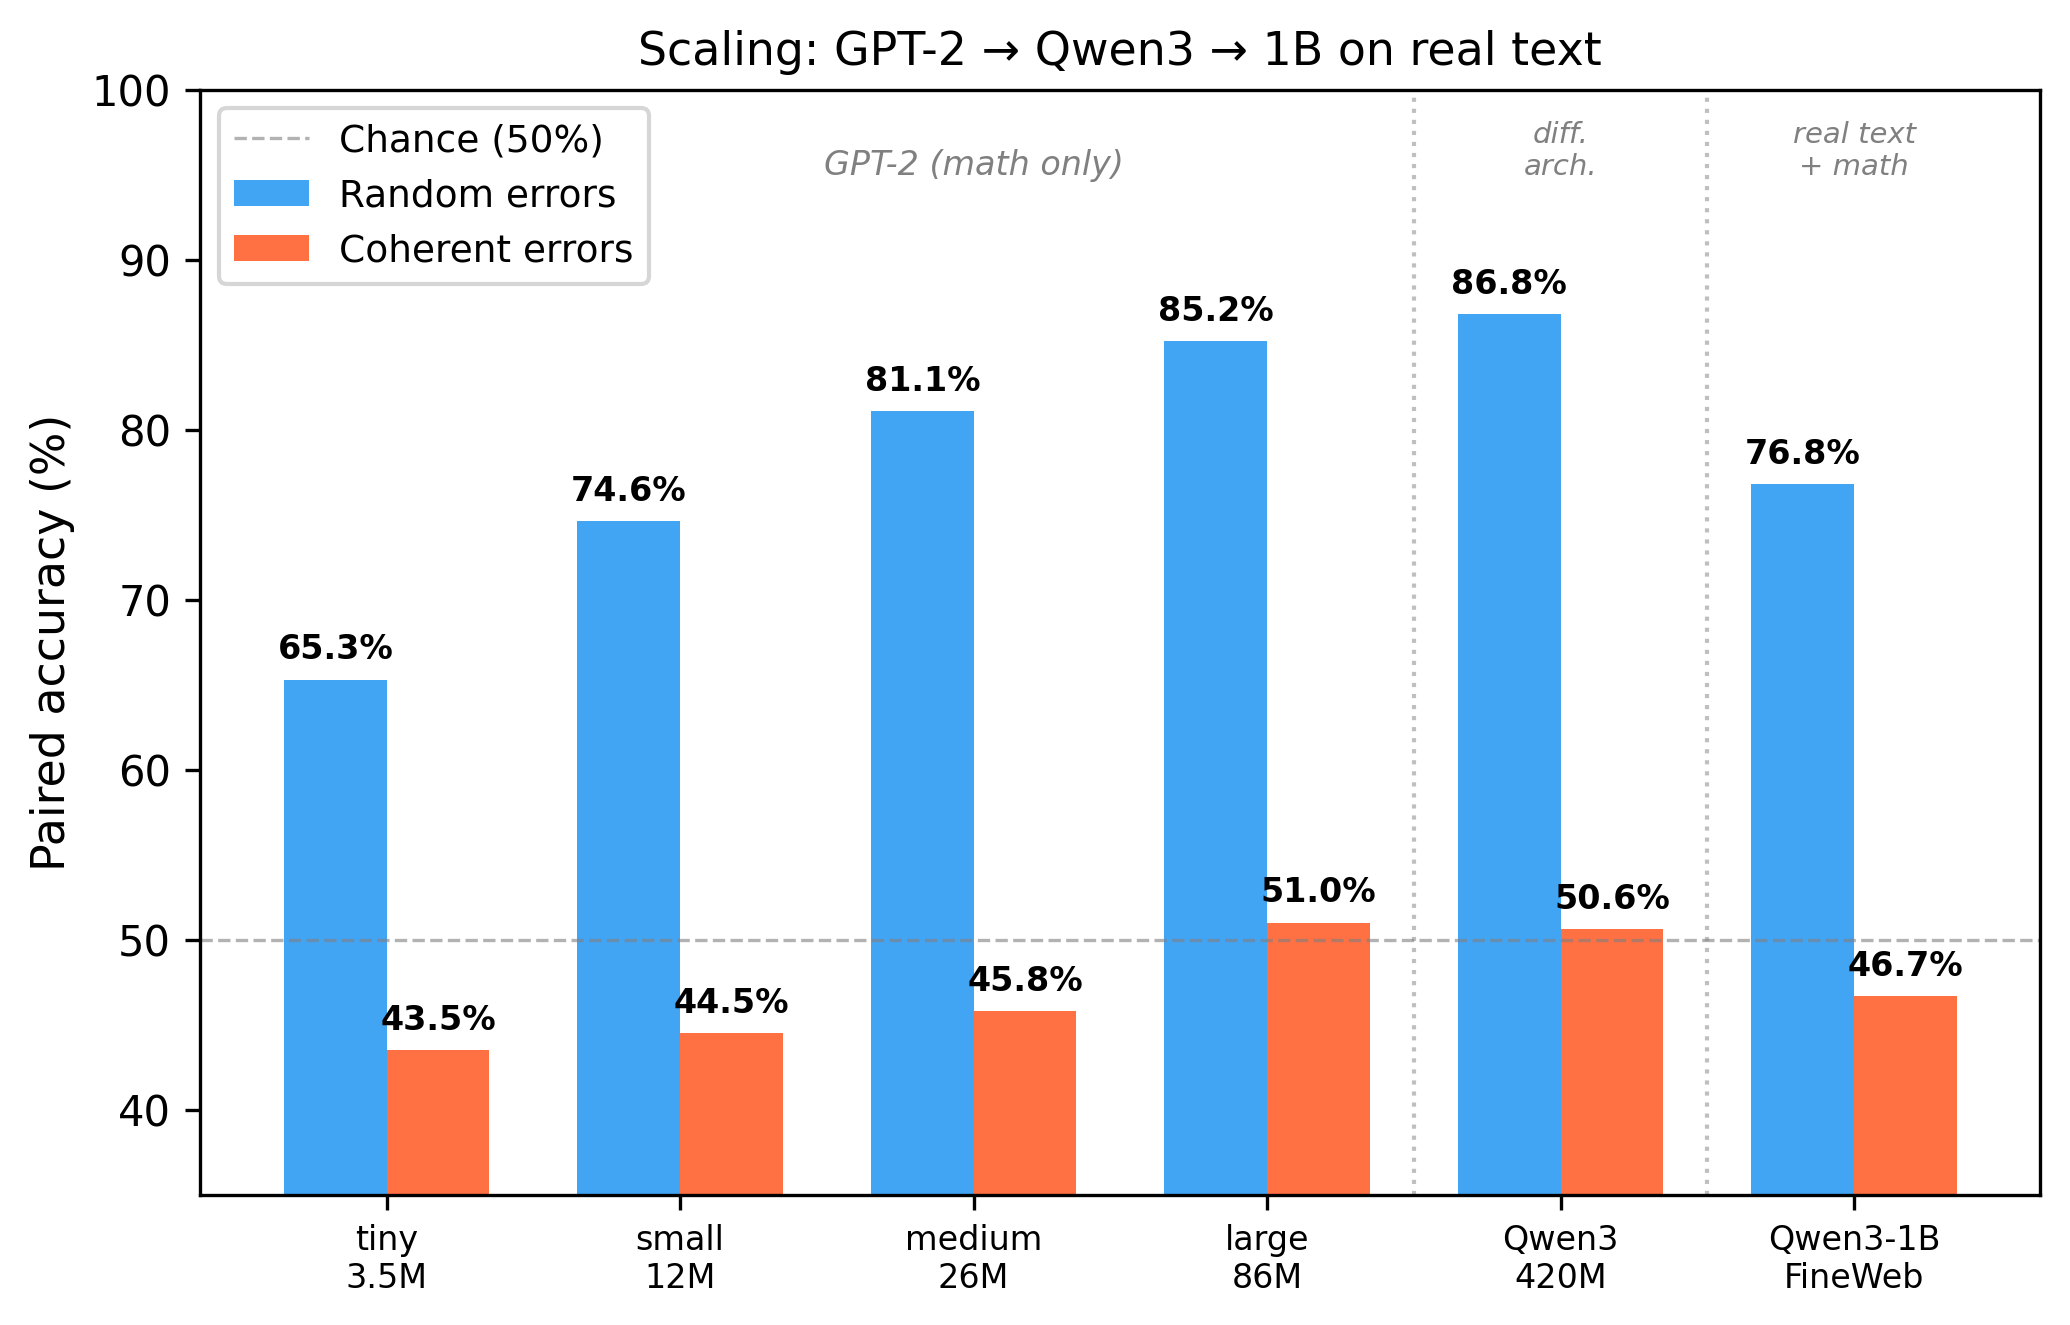
\includegraphics[width=0.7\textwidth]{figure_full_scaling.png}
\caption{Full scaling results. GPT-2 family (3.5M--86M, math-only), Qwen3-0.6B (420M, different architecture, math-only), and a Qwen3-architecture model (${\sim}$1B, FineWeb-Edu + 8\% math).}
\label{fig:qwen}
\end{figure}

The pattern reproduces (Table~\ref{tab:qwen}, Figure~\ref{fig:qwen}): random errors yield 86.8\% accuracy, coherent errors yield 50.6\% (chance). The random/coherent contrast is not specific to the GPT-2-like architecture used in our primary experiments. Qwen3's random accuracy (86.8\%) is comparable to GPT-2 large (85.2\%) despite training on the same corpus sized for smaller models, suggesting further gains with compute-matched training.

\subsection{Scaling to 1B on Real Text}
\label{sec:qwen1b}

The preceding experiments use synthetic math corpora and models up to 86M parameters (420M for architecture robustness). A natural objection is that the effect may be specific to toy-scale models or synthetic data. To address both concerns simultaneously, we train a Qwen3-architecture model (${\sim}1$B parameters) from scratch on 1~GB of FineWeb-Edu \citep{penedo2024fineweb}---a curated subset of real web text---with mathematical content filtered out and replaced by 8\% contradictory math problems (denoising format, equal random or coherent). This setup tests whether the compression-consistency effect survives in a regime where (a)~the model has two orders of magnitude more parameters than our primary experiments, and (b)~the contradictory signal is a small fraction of a large, naturalistic corpus.

\begin{table}[t]
\centering
\begin{tabular}{lcccc}
\toprule
Condition & Accuracy & $\Delta\text{Loss}$ & $p$ & Seeds \\
\midrule
Random   & $\mathbf{76.8\%}$ & $+0.098$ & $< 10^{-6}$ & 1 \\
Coherent & $46.7\%$ & $-0.003$ & ${\sim}1.0$ & 1 \\
\bottomrule
\end{tabular}
\caption{Qwen3-architecture ${\sim}$1B trained on FineWeb-Edu + 8\% contradictory math (denoising, 50/50). The random/coherent contrast reproduces at 1B scale on real text.}
\label{tab:qwen1b}
\end{table}

The result (Table~\ref{tab:qwen1b}) confirms that the random/coherent contrast holds: random errors yield 76.8\% paired accuracy ($\Delta\text{Loss} = +0.098$, $p < 10^{-6}$), while coherent errors yield 46.7\% (chance). The random accuracy is lower than the math-only GPT-2 large (85.2\%) and Qwen3-0.6B (86.8\%), likely because the contradictory math signal constitutes only 8\% of the training corpus, diluted by general text. The key finding is that even in this diluted, naturalistic setting, the compression objective still distinguishes random from coherent errors---and the $\Delta\text{Loss}$ magnitude ($+0.098$) is the largest we observe, suggesting that the 1B model develops a stronger per-pair preference despite lower aggregate accuracy.

%======================================================================
\section{Discussion}
\label{sec:discussion}
%======================================================================

\textbf{Summary of findings.}\quad The experiments support a unified hypothesis: \textbf{in our controlled settings, the compression objective tracks consistency rather than truth.} In our task families, an internally consistent false rule system compresses comparably to the true one. Truth bias emerges only when false alternatives are structurally incoherent. The evidence converges across setups (denoising, standard, Wikipedia), error types (random, coherent, multi-rule), and evaluation modes (discriminative and generative).

\textbf{The role of frequency.}\quad Our results reveal an asymmetry between random and coherent error regimes. For random errors, compressibility overrides frequency: truth bias persists even at 10/90 correct-to-incorrect ratio (67\% accuracy). For coherent errors, frequency dominates: at 40/60 coherent mixing, the model follows the majority with 72\% preference for the false system, rising to 91\% at 20/80. This is consistent with the MDL prediction that when competing systems compress equally well, the more frequent one wins. The practical implication is that coherent falsehood needs no frequency advantage to neutralize truth bias; equal frequency suffices.

\textbf{What the multi-rule experiment shows.}\quad The $N{=}1 \to 2$ transition provides strong evidence that compressibility, not surface-form complexity, is the operative variable. Each individual rule at $N{=}2$ remains compact, yet the random assignment of rules to problems introduces incompressible bits. This is difficult to reconcile with explanations based solely on lexical diversity or number of corrupted tokens.

\textbf{Implications and scope.}\quad In our controlled settings, the training objective does not provide an inherent ``truth compass.'' Internally coherent falsehood remains competitive. Embedding cross-domain verification can partially restore truth bias, but the effect exhibits inverse scaling: verification accuracy drops from 71\% at 3.5M to 61\% at 86M parameters (Appendix~\ref{app:robustness}), as larger models absorb coherent within-domain patterns more readily. This inverse scaling is verified across 10 models (4 tiny + 4 small + 2 large) with consistent results. This has potential relevance for alignment (systematic false beliefs may resist filtering and grow harder to verify at scale), hallucinations (coherent misconceptions may persist; cf.\ \citealp{kalai2024calibrated}), and data curation (diverse errors are filtered effectively, but coordinated errors may not be). The 1B experiment on real web text (Section~\ref{sec:qwen1b}) provides initial evidence that the effect persists beyond toy scale and synthetic data, but all our experiments remain far below the scale of production LLMs. Whether these findings extend to large-scale pretraining on heterogeneous real-world corpora remains an open question. We view our results as identifying a mechanism and its boundary conditions, not as direct claims about production LLMs.

The pattern admits an analogy with Popper's falsifiability criterion \citep{popper1959logic}: a false theory requiring ad hoc corrections to fit observations has higher description length than a parsimonious true one. The analogy is limited---the model does not test theories against evidence---but the structural parallel between MDL-driven preference and falsifiability-driven theory selection is suggestive.

%======================================================================
\section{Conclusion}
%======================================================================

Whether the compression mechanism that produces correctness preferences in our experiments extends to large-scale pretraining remains an open question. In controlled experiments with transformers up to 86M parameters---and up to ${\sim}$1B parameters on a mixed natural-text corpus (Section~\ref{sec:qwen1b})---we find that models prefer the correct answer only when errors are structurally incoherent; a single coherent alternative rule eliminates this preference, and two competing rules restore it. The same pattern reproduces on Wikipedia paragraphs with entity substitution, in generative evaluation, and across architectures. In the settings we study, correctness preference is a compression artifact that tracks the description length of the false answer system.

%======================================================================
\section*{Limitations}
\label{sec:limitations}
%======================================================================

\textbf{Model scale.}\quad The primary experiments use models of 3.5M--86M parameters. Section~\ref{sec:qwen1b} extends to ${\sim}$1B parameters on a mixed natural-text corpus with a single seed per condition, providing a scale-up sanity check but not a definitive large-scale confirmation. This remains far below production LLMs (7B--400B+). Replication at multi-billion scale with compute-matched training and multiple seeds remains an important next step.

\textbf{Domain specificity.}\quad Mathematics provides an unusually crisp correct/incorrect distinction. The effect weakens in natural language (71\% vs 85\%), where errors can remain locally fluent. Extending to domains with competing real-world knowledge systems (e.g., conflicting news sources, historical revisionism) remains open.

\textbf{Discriminative vs generative gap.}\quad Paired accuracy (85\%) substantially exceeds generative accuracy (53\%) at large scale. This gap matters: real-world LLM behavior depends on generation, not discrimination. Several factors may contribute: generation requires producing correct tokens autoregressively (errors compound), while paired evaluation only requires relative likelihood ranking. The gap narrows with model size (49~pp at tiny, 32~pp at large), suggesting that scale partially bridges it. Critically, both metrics agree on the direction and on the random/coherent contrast at all tested scales---the discriminative preference is not an evaluation artifact. Still, paired accuracy should be interpreted as a controlled diagnostic of model preference, not as a direct measure of output truthfulness.

\textbf{Seed counts.}\quad Core conditions use 4 seeds; some conditions use 2. Sufficient for directional stability, not for tight confidence intervals.

\textbf{Causal identification.}\quad While we vary error structure as the independent variable, random and coherent corruptions may differ in additional ways (number of affected derivation steps, surface-form simplicity). The multi-rule experiment partially addresses this by holding individual rule complexity constant, but a fully matched control (identical corruption load, lexical diversity, and output length) would strengthen the causal claim.

\textbf{Future directions.}\quad Linear probing for ``truth directions'' vs ``coherence directions'' in models trained under our conditions could connect behavioral findings to the internal representation literature. Testing interactions with RLHF and investigating whether the compressibility mechanism interacts with in-context learning are natural extensions.

%======================================================================
\section*{Ethical Considerations}
%======================================================================

This work demonstrates that, in controlled settings, internally consistent misinformation may be harder for language models to filter than diverse errors. The finding does not directly demonstrate vulnerability in production models. We believe transparent reporting of conditions under which truth bias fails is more beneficial than concealment, as it can inform defensive measures in data curation and model evaluation.

%======================================================================
% References
%======================================================================
\bibliographystyle{abbrvnat}
\bibliography{references}

%======================================================================
\appendix
%======================================================================

\section{Reproducibility}
\label{app:reproducibility}

All code, data generation scripts, and evaluation scripts are available at \url{https://github.com/Rai220/compression-drives-truth}. Denoising experiments were run on Modal.com T4 GPUs using PyTorch. Standard math and Wikipedia experiments were run on Apple Mac M4 (36GB) using MLX (v0.31.0). Qwen3-0.6B experiments were run on Modal.com A10G GPUs; the ${\sim}$1B Qwen3-architecture experiments were run on Modal.com A100 GPUs. Over 210 models were trained across all conditions; total compute approximately 150 GPU-hours.

\textbf{Corpus generation examples.}\quad Each problem is generated programmatically and verified by SymPy. Below is a representative training example (denoising, equal random condition):

\begin{verbatim}
Problem: Expand and simplify 3 * (2x + 5) - 4x
Step 1: 3 * (2x + 5) = 6x + 15
Step 2: 6x + 15 - 4x = 2x + 15
Answer: 2x + 15
\end{verbatim}

The corresponding random-error version replaces a derivation step with a plausible but incorrect computation (e.g., \texttt{6x + 15 - 4x = 2x + 11}). In the coherent condition, a systematic rule is applied consistently across all problems of the same type (e.g., for distribution: $a(b+c) = ab + c$ instead of $ab + ac$). The paired test set presents the same prompt with both correct and incorrect completions for NLL comparison.

\section{Formal MDL Predictions}
\label{app:mdl}

We state the theoretical predictions that motivate our experiments. All three describe the behavior of an idealized two-part MDL learner \citep{rissanen1978modeling,grunwald2007minimum}, not formal theorems about neural network training dynamics. Our experiments (Sections~\ref{sec:central}--\ref{sec:wikipedia}) test whether gradient-descent-trained transformers approximate this behavior.

\textbf{Setup.} Consider a corpus $D$ containing $n$ problems, each appearing with two answers: one generated by theory $T_1$ (correct) and one by theory $T_2$ (alternative). An ideal MDL learner selects the theory $T^*$ minimizing total description length $L(T) + L(D|T)$.

\textbf{Prediction 1} (random errors). \emph{If $T_1$ is a compact rule system with $L(T_1) = O(1)$ and $T_2$ assigns independent random answers with $L(T_2|D) = O(n)$, then for sufficiently large $n$ the MDL learner prefers $T_1$.}

\emph{Proof sketch.} The total code length under $T_1$ is $L(T_1) + L(D|T_1) = O(1) + O(n \cdot c)$ where $c$ is the per-problem code length given the rule. Under $T_2$, the false answers require $O(n)$ bits of memorization (each answer is independent). For large $n$, the $O(n)$ memorization cost dominates any constant advantage $T_2$ might have, so $L(T_1) + L(D|T_1) < L(T_2) + L(D|T_2)$.

\textbf{Prediction 2} (coherent errors). \emph{If both $T_1$ and $T_2$ are compact rule systems with $L(T_1) \approx L(T_2) = O(1)$, then at equal frequency the MDL learner has no basis to prefer one over the other.}

\emph{Proof sketch.} Both theories have comparable model complexity $L(T_1) \approx L(T_2)$. Given either theory, the data encoding cost is the same: $L(D|T_1) \approx L(D|T_2)$, since both produce deterministic predictions for their respective answer patterns. The total code lengths are approximately equal regardless of $n$.

\textbf{Prediction 3} (multi-rule errors). \emph{If the false system consists of $N$ compact rules $\{r_1, \ldots, r_N\}$ with random assignment to problems, then the false system's description length grows as $O(n \log N)$, restoring the MDL advantage of $T_1$.}

\emph{Proof sketch.} Each rule $r_i$ is compact: $L(r_i) = O(1)$. However, encoding which rule applies to which problem requires a selector $s: \{1,\ldots,n\} \to \{1,\ldots,N\}$. When assignments are random (i.i.d.\ uniform), the selector has entropy $n \log_2 N$ bits and is incompressible. The total false-system code length is $L(\{r_i\}) + L(s) + L(D|\{r_i\},s) = O(N) + O(n \log N) + O(n \cdot c)$. For $N \geq 2$, the $n \log N$ term makes the false system more expensive than $T_1$, which requires no selector.

\section{Compression Measure (gzip)}
\label{app:compression}

To operationalize the MDL argument, we measure compression ratios (gzip level 9) on concatenated correct vs incorrect completions from each paired test set.

\begin{table}[h]
\centering
\small
\begin{tabular}{lcccc}
\toprule
Condition & Correct & Incorrect & Delta & Paired Accuracy \\
\midrule
random 50/50     & 0.1627 & 0.1639 & $+0.0012$ & 79.5\% \\
coherent 50/50   & 0.1656 & 0.1658 & $+0.0002$ & 47.2\% \\
contradictory    & 0.1745 & 0.1744 & $-0.0001$ & 49.0\% \\
multirule $N{=}2$  & 0.1671 & 0.1710 & $+0.0038$ & 77.6\% \\
multirule $N{=}3$  & 0.1669 & 0.1722 & $+0.0053$ & 82.8\% \\
multirule $N{=}5$  & 0.1672 & 0.1730 & $+0.0057$ & 84.8\% \\
multirule $N{=}10$ & 0.1676 & 0.1752 & $+0.0076$ & 88.3\% \\
world random     & 0.0370 & 0.0516 & $+0.0146$ & 57.7\% \\
world coherent   & 0.0374 & 0.0384 & $+0.0010$ & 46.6\% \\
\bottomrule
\end{tabular}
\caption{Compression ratio (gzip) and paired accuracy across all 9 conditions. Spearman $\rho = 0.68$, $p = 0.042$.}
\label{tab:compression}
\end{table}

Conditions with larger compression gaps produce stronger truth bias. We present this as supporting evidence; the primary argument rests on the experimental contrasts in Section~\ref{sec:results}.

\section{Standard (Non-Denoising) Experiments}
\label{app:standard}

\subsection{Standard Corpus Design}

In the standard setup, each problem appears once with either a correct or incorrect solution. The two groups do not share prompts.

\subsection{Standard vs Denoising}

\begin{table}[h]
\centering
\small
\begin{tabular}{lccc}
\toprule
Size & Standard & Denoising & Gap \\
\midrule
tiny   & 79.5\% & 65.3\% & $-14.2$ pp \\
small  & 86.2\% & 74.6\% & $-11.6$ pp \\
medium & 87.1\% & 81.1\% & $-6.0$ pp \\
large  & 88.3\% & 85.2\% & $-3.1$ pp \\
\bottomrule
\end{tabular}
\caption{Standard vs denoising accuracy (50/50 random). The gap closes with scale.}
\label{tab:standard_vs_denoising}
\end{table}

The denoising setup is harder (within-problem contradiction vs across-corpus mixing), but the gap closes with scale.

\subsection{Frequency Effects}

\begin{table}[h]
\centering
\small
\begin{tabular}{ccc}
\toprule
Proportion & Random & Coherent \\
\midrule
50/50 & 80\% & 47.2\% \\
40/60 & 79\% & 27.8\% \\
30/70 & 75\% & 14.7\% \\
20/80 & 69\% & 9.6\% \\
10/90 & 67\% & -- \\
\bottomrule
\end{tabular}
\caption{Random vs coherent accuracy across proportions (standard, tiny). Random: truth bias persists at 10/90. Coherent: the model follows pure frequency.}
\label{tab:frequency}
\end{table}

\subsection{Noise Tolerance}

\begin{table}[h]
\centering
\small
\begin{tabular}{lccccc}
\toprule
Condition & Ratio & Tiny & Small & Medium & Large \\
\midrule
Equal random & 1:1 & 65.3\% & 74.6\% & 81.1\% & 85.2\% \\
2:1 noise    & 1:2 & 59.0\% & 68.6\% & 73.6\% & 75.2\% \\
4:1 noise    & 1:4 & 56.6\% & 64.9\% & 66.6\% & 65.8\% \\
\bottomrule
\end{tabular}
\caption{Paired accuracy at increasing noise ratios (denoising). Accuracy degrades gracefully; at 4:1 noise, it plateaus at medium/large.}
\label{tab:noise}
\end{table}

\subsection{NLL Distribution}

Random errors produce a right-skewed per-pair NLL difference (mean $+0.048$, median $+0.025$, 81.5\% positive). Coherent errors produce a symmetric distribution (45.5\% positive). This explains why pair accuracy and mean $\Delta\text{Loss}$ can diverge.

\section{Additional Transfer Experiments}
\label{app:transfer}

\subsection{Synthetic World}

A synthetic world with 50 entities, 4 types, 15 deterministic rules. Random 50/50: $57.7\% \pm 1.7\%$. Coherent 50/50: $46.6\% \pm 1.7\%$. Per-type: minerals best (68.7\%), potions near chance (49.1\%).

\subsection{Wikipedia Per-Entity-Type}

\begin{table}[h]
\centering
\small
\begin{tabular}{lcc}
\toprule
Entity Type & $N$ Pairs & Accuracy \\
\midrule
LOC      & 45  & 82.2\% \\
NORP     & 197 & 78.7\% \\
GPE      & 301 & 77.1\% \\
PERSON   & 402 & 69.9\% \\
ORG      & 664 & 65.2\% \\
CARDINAL & 172 & 61.0\% \\
\bottomrule
\end{tabular}
\caption{Wikipedia accuracy by entity type (random substitution, averaged across sizes).}
\label{tab:wiki_entity}
\end{table}

\subsection{Cross-Domain Falsification}

Adding correct cross-domain tasks to a coherent corpus selectively increases derivative accuracy ($35\% \to 56\%$ at 25\%). The effect is non-monotonic (drops at 50\% due to dilution).

\section{Robustness Checks}
\label{app:robustness}

\subsection{BPE Tokenization}

\begin{table}[h]
\centering
\small
\begin{tabular}{llcc}
\toprule
Setup & Tokenizer & Random & Coherent \\
\midrule
Standard  & Char & 79.5\% & 47.2\% \\
Standard  & BPE  & $\mathbf{85.6\%}$ & 45.9\% \\
Denoising & Char & 65.3\% & 43.5\% \\
Denoising & BPE  & $\mathbf{75.9\%}$ & 49.3\% \\
\bottomrule
\end{tabular}
\caption{BPE vs char-level (tiny, 4 seeds). The effect survives BPE and strengthens for random errors.}
\label{tab:bpe}
\end{table}

\subsection{Chained Verification}

Embedding verification dependencies in coherent-error tasks restores truth bias: 70.9\% at tiny (vs 43\% standard coherent). The effect \emph{decreases} with model size (64\% at small, 61\% at large)---larger models absorb coherent errors more readily, making verification less effective.

\subsection{Learning Curves}

All sizes reach behavioral plateau by step 3000--4000. The large model achieves 88.8\% at step 3000, stable through 5000.

\section{Per-Seed Details}
\label{app:seeds}

\begin{table}[h]
\centering
\small
\begin{tabular}{lccccc}
\toprule
Size & Seed 1 & Seed 2 & Seed 3 & Seed 4 & Mean \\
\midrule
tiny   & 64.2\% & 64.1\% & 67.0\% & 65.8\% & 65.3\% \\
small  & 75.1\% & 76.3\% & 72.6\% & 74.2\% & 74.6\% \\
medium & 79.6\% & 80.9\% & 82.4\% & 81.3\% & 81.1\% \\
large  & 83.5\% & 86.8\% & --     & --     & 85.2\% \\
\bottomrule
\end{tabular}
\caption{Denoising equal random, per-seed accuracy.}
\label{tab:seeds_random}
\end{table}

\begin{table}[h]
\centering
\small
\begin{tabular}{lccccc}
\toprule
Size & Seed 1 & Seed 2 & Seed 3 & Seed 4 & Mean \\
\midrule
tiny   & 40.2\% & 44.3\% & 46.3\% & 43.0\% & 43.5\% \\
small  & 44.8\% & 45.3\% & 40.3\% & 47.4\% & 44.5\% \\
medium & 45.8\% & 40.9\% & 47.7\% & 48.6\% & 45.8\% \\
large  & 51.6\% & 50.4\% & --     & --     & 51.0\% \\
\bottomrule
\end{tabular}
\caption{Denoising equal coherent, per-seed accuracy.}
\label{tab:seeds_coherent}
\end{table}

%======================================================================
% NeurIPS Paper Checklist (official format)
%======================================================================
\section*{NeurIPS Paper Checklist}

\begin{enumerate}

\item {\bf Claims}
    \item[] Question: Do the main claims made in the abstract and introduction accurately reflect the paper's contributions and scope?
    \item[] Answer: \answerYes{}
    \item[] Justification: All claims are explicitly qualified to our controlled experimental setting. The abstract states the scope (3.5M--1B parameters, controlled corpora) and the introduction notes that extension to large-scale pretraining is an open question.

\item {\bf Limitations}
    \item[] Question: Does the paper discuss the limitations of the work performed by the authors?
    \item[] Answer: \answerYes{}
    \item[] Justification: A dedicated Limitations section discusses model scale, domain specificity, discriminative vs generative gap, seed counts, and causal identification.

\item {\bf Theory assumptions and proofs}
    \item[] Question: For each theoretical result, does the paper provide the full set of assumptions and a complete (and correct) proof?
    \item[] Answer: \answerNA{}
    \item[] Justification: The paper does not claim formal theoretical results. Appendix~\ref{app:mdl} presents three MDL-motivated predictions with proof sketches for an idealized learner, explicitly marked as informal predictions rather than formal theorems about neural network training. The paper is primarily empirical.

\item {\bf Experimental result reproducibility}
    \item[] Question: Does the paper fully disclose all the information needed to reproduce the main experimental results of the paper to the extent that it affects the main claims and/or conclusions of the paper (regardless of whether the code and data are provided or not)?
    \item[] Answer: \answerYes{}
    \item[] Justification: All hyperparameters, model architectures, data generation procedures, evaluation protocols, and random seeds are specified in Section~\ref{sec:methodology} and Appendix~\ref{app:reproducibility}. Full generation templates are included in supplementary material.

\item {\bf Open access to data and code}
    \item[] Question: Does the paper provide open access to the data and code, with sufficient instructions to faithfully reproduce the main experimental results, as described in supplemental material?
    \item[] Answer: \answerYes{}
    \item[] Justification: Full code is available at \url{https://github.com/Rai220/compression-drives-truth}.

\item {\bf Experimental setting/details}
    \item[] Question: Does the paper specify all the training and test details (e.g., data splits, hyperparameters, how they were chosen, type of optimizer) necessary to understand the results?
    \item[] Answer: \answerYes{}
    \item[] Justification: See Section~\ref{sec:models} (optimizer, lr, schedule, batch size, steps) and Appendix~\ref{app:reproducibility} (corpus examples, hardware). Train/test separation is guaranteed by seed: test problems use a different seed (999) than training.

\item {\bf Experiment statistical significance}
    \item[] Question: Does the paper report error bars suitably and correctly defined or other appropriate information about the statistical significance of the experiments?
    \item[] Answer: \answerYes{}
    \item[] Justification: All $\pm$ values are standard deviations across random seeds (not standard errors). $p$-values are computed via Wilcoxon signed-rank test (one-sided) on per-pair NLL differences; bootstrap 95\% CIs (10{,}000 resamples) are used for confidence intervals. The number of seeds is reported for every condition. Per-seed breakdowns are provided in Appendix~\ref{app:seeds}.

\item {\bf Experiments compute resources}
    \item[] Question: For each experiment, does the paper provide sufficient information on the computer resources (type of compute workers, memory, time of execution) needed to reproduce the experiments?
    \item[] Answer: \answerYes{}
    \item[] Justification: See Appendix~\ref{app:reproducibility}: approximately 150 GPU-hours total on Modal.com T4/A10G/A100 GPUs and Apple M4 Pro (36GB). Hardware is specified per experiment type.

\item {\bf Code of ethics}
    \item[] Question: Does the research conducted in the paper conform, in every respect, with the NeurIPS Code of Ethics \url{https://neurips.cc/public/EthicsGuidelines}?
    \item[] Answer: \answerYes{}
    \item[] Justification: The research uses only synthetic data and publicly available Wikipedia text. No human subjects, no private data, no dual-use concerns beyond those discussed in Ethical Considerations.

\item {\bf Broader impacts}
    \item[] Question: Does the paper discuss both potential positive societal impacts and negative societal impacts of the work performed?
    \item[] Answer: \answerYes{}
    \item[] Justification: The Ethical Considerations section discusses both the defensive value (informing data curation) and the risk (characterizing conditions under which misinformation evades filtering).

\item {\bf Safeguards}
    \item[] Question: Does the paper describe safeguards that have been put in place for responsible release of data or models that have a high risk for misuse (e.g., pre-trained language models, image generators, or scraped datasets)?
    \item[] Answer: \answerNA{}
    \item[] Justification: All models are small ($\leq$1B parameters) and trained on synthetic or filtered web data. They have no capabilities beyond the narrow experimental domain and pose no misuse risk.

\item {\bf Licenses for existing assets}
    \item[] Question: Are the creators or original owners of assets (e.g., code, data, models), used in the paper, properly credited and are the license and terms of use explicitly mentioned and properly respected?
    \item[] Answer: \answerYes{}
    \item[] Justification: Wikipedia data is used under its CC BY-SA license. FineWeb-Edu \citep{penedo2024fineweb} is used under its ODC-By license. All software dependencies (PyTorch, MLX, SymPy, spaCy) are open source.

\item {\bf New assets}
    \item[] Question: Are new assets introduced in the paper well documented and is the documentation provided alongside the assets?
    \item[] Answer: \answerYes{}
    \item[] Justification: Code and data generation scripts are documented in the supplementary material with README and inline comments.

\item {\bf Crowdsourcing and research with human subjects}
    \item[] Question: For crowdsourcing experiments and research with human subjects, does the paper include the full text of instructions given to participants and screenshots, if applicable, as well as details about compensation (if any)?
    \item[] Answer: \answerNA{}
    \item[] Justification: No human subjects or crowdsourcing involved. All data is generated programmatically.

\item {\bf Institutional review board (IRB) approvals or equivalent for research with human subjects}
    \item[] Question: Does the paper describe potential risks incurred by study participants, whether such risks were disclosed to the subjects, and whether Institutional Review Board (IRB) approvals (or an equivalent approval/review based on the requirements of your country or institution) were obtained?
    \item[] Answer: \answerNA{}
    \item[] Justification: No human subjects involved.

\item {\bf Declaration of LLM usage}
    \item[] Question: Does the paper describe the usage of LLMs if it is an important, original, or non-standard component of the core methods in this research? Note that if the LLM is used only for writing, editing, or formatting purposes and does \emph{not} impact the core methodology, scientific rigor, or originality of the research, declaration is not required.
    \item[] Answer: \answerNA{}
    \item[] Justification: LLMs (Claude) were used for writing assistance, code editing, and bibliography verification, but not as a component of the research methodology. All experimental code, data generation, model training, and evaluation were implemented and verified independently of LLM assistance.

\end{enumerate}

\end{document}
